%ch2.tex
\chapter{Continuous Probability Densities}
\section{Simulations of Continuous Probabilities}
The code solutions for  \href{https://github.com/krishramkumar06/probability/tree/main/grinstead_snell_probability_solutions/ch2/2-1}{section 2.1} are linked and posted on my github repository.

\section{Continuous Density Functions}

The code solutions for  \href{https://github.com/krishramkumar06/probability/tree/main/grinstead_snell_probability_solutions/ch2/2-2}{section 2.2} are linked and posted on my github repository.

\begin{oddenumerate}
	\item (a) $ \frac{b-a}{8} $ (b) i. $ 5/8 $, ii. $ 2/8 $, iii. $ (3 + 3)/8 = 6/8 $
	\item (a) $\displaystyle  1 = C\int_2^{10} \frac{\textrm{dx}}{x} \implies C = \log(2)/\log(10)$. (b) $ (\log(2)/\log(10))(\log(b)/\log(a)) $. (c) i.  $ (\log(2)/\log(10))(\log(10)/\log(5)) $, ii. $ (\log(2)/\log(10))(\log(7)/\log(2)) $ iii. $ (\log(2)/\log(10))((\log(5)/\log(2)) + (\log(10)/\log(7)))$
	\item (a) $ 1 - e^{-1} $. (b) $ 1 - e^{-3} $. (c) $ e^{-3} - e^{-4} $ .(d) $ e^{-4}$
	\item (a) $ 1/3 $. (b) $ 1/2 $. (c) $ 1/2 $ (d) $ 1/3 $
	\item Since the exponential density is memoryless, we would expect the average time to still be 10 minutes after 100 minutes have passed. This was confirmed by the simulated time of 9.65
	\item Wait Time after 100:  72.87715443485199. It's barely possible for the 3 to get over 100.
	\item This one is a really important problem so I will give it extra special care: ``Take a stick of unit length and break it into two pieces, choosing the break point at random. Now break the longer of the two pieces at a random point.
	What is the probability that the three pieces can be used to form a triangle?"
	\\ Assume (because of symmetry) that $ X $ is uniformly distributed from $ [0, 1/2] $ as this will ensure that $ 1-X $ is the longer stick which is being broken, meaning that $ Y $ is uniformly distributed on $ [0, 1-X] $.  Our PDFs are 
	\begin{align*}
		f_X(x) &= 2
		\\ f_{Y|X}(y|x) &= 1/(1-X)
	\end{align*}
	We use a marginal and a conditional PDF and use the multiplication rule to obtain the joint PDF
	\[ f_{Y|X}(y|x) * f_X(x)  = f_{X,Y}(x,y) = \frac{2}{1-x} \]
	To make a triangle, we must satisfy the triangle inequality
	\begin{align*}
		X + Y > 1 - X - Y \implies Y &> \half - X
		\\ 1 - X - Y + Y > X \implies X &< \half
		\\ 1 - X - Y + X > Y \implies Y &< \half
	\end{align*}
	This means we need to find $ P(X \leq 1/2, Y \in [\half - X, \half]) $. This is the integral expression
	 \begin{align*}
	 		 \displaystyle \int_0^{\half} \int_{\half - X}^{\half} f_{X,Y}(x,y) \textrm{ dxdy} &= \displaystyle \int_0^{\half} \int_{\half - x}^{\half} \frac{2}{1-x}  \textrm{ dxdy}   
	 		 \\ &= \int_0^\half \dfrac{2(\half - (\half - x))}{1 - x} \textrm{dx}
			 \\ &= \int_0^\half \dfrac{2x}{1 - x} \textrm{dx}
			 \\ &= 2\int_1^\half \dfrac{(1 - u)}{u} \textrm{du}
			 \\ &= 2\int_\half^1 \dfrac{1}{u}  - 1\textrm{du}
			  \\ &= 2\int_\half^1 \dfrac{1}{u}  - 1\textrm{du}
			  \\ &= 2\log(2) - 1 \approx \boxed{0.386}
	 \end{align*}
 	Please note that joint PDFs and conditional PDFs are introduced in chapter 4 and the multiplication rule is not introduced at all. Tricks in symmetry can be used to handwave to a solution.
 	\item Yes, its fair as your expected winnings is the same as the amount you pay to enter.
 	\item Fraction that $ X>5 $:  $ 0.643 $
 	Fraction that $ 5<X<7 $:  $ 0.274 $
 	Fraction that $ x^2 - 12x + 35 > 0  $: $  0.726 $
 	var1:  $ 0.018 $
 	var2:  $ 0.024 $
 	var3:  $ -0.024$
 	\item Fraction that cond1:  0.324
 	Fraction that cond2:  0.487
 	Fraction that cond3:  0.513
 	Fraction that cond4:  0.343
 	var1:  -0.009333
 	var2:  -0.013000
 	var3:  0.0130000
 	var4:  0.0096666
 	\item probTriangle:  0.4992
 	\item 
\begin{center}
	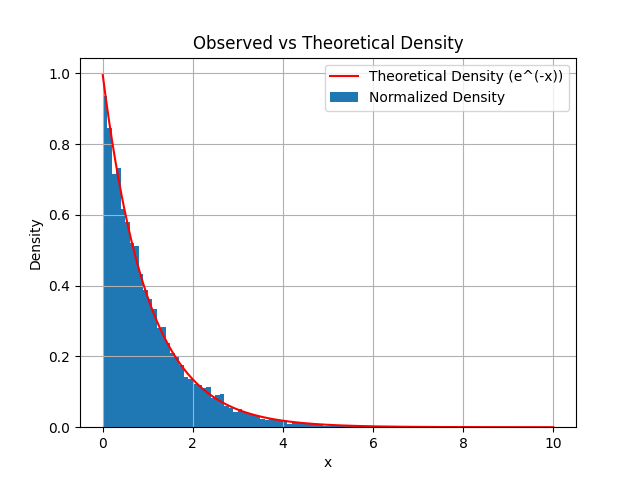
\includegraphics[width=0.8\linewidth]{../../../probability/grinstead_snell_probability_solutions/ch2/2-2/plot2-2-23}
\end{center}
\end{oddenumerate}